\section{Durchführung}
\noindent Die Schaltungen werden entsprechend der Schaltskizzen \ref{fig:03} bis
\ref{fig:07} auf der Steckplatine wie in \autoref{aufbau} dargestellt
aufgesteckt. Zu beachten ist dabei, dass die Schaltungen erst mit Spannung
versorgt werden, wenn die Widerstände dem Operationsverstärker vorgeschaltet
sind, um Schäden am elektrischen Bauteil zu vermeiden. \\
\begin{figure}
  \centering
  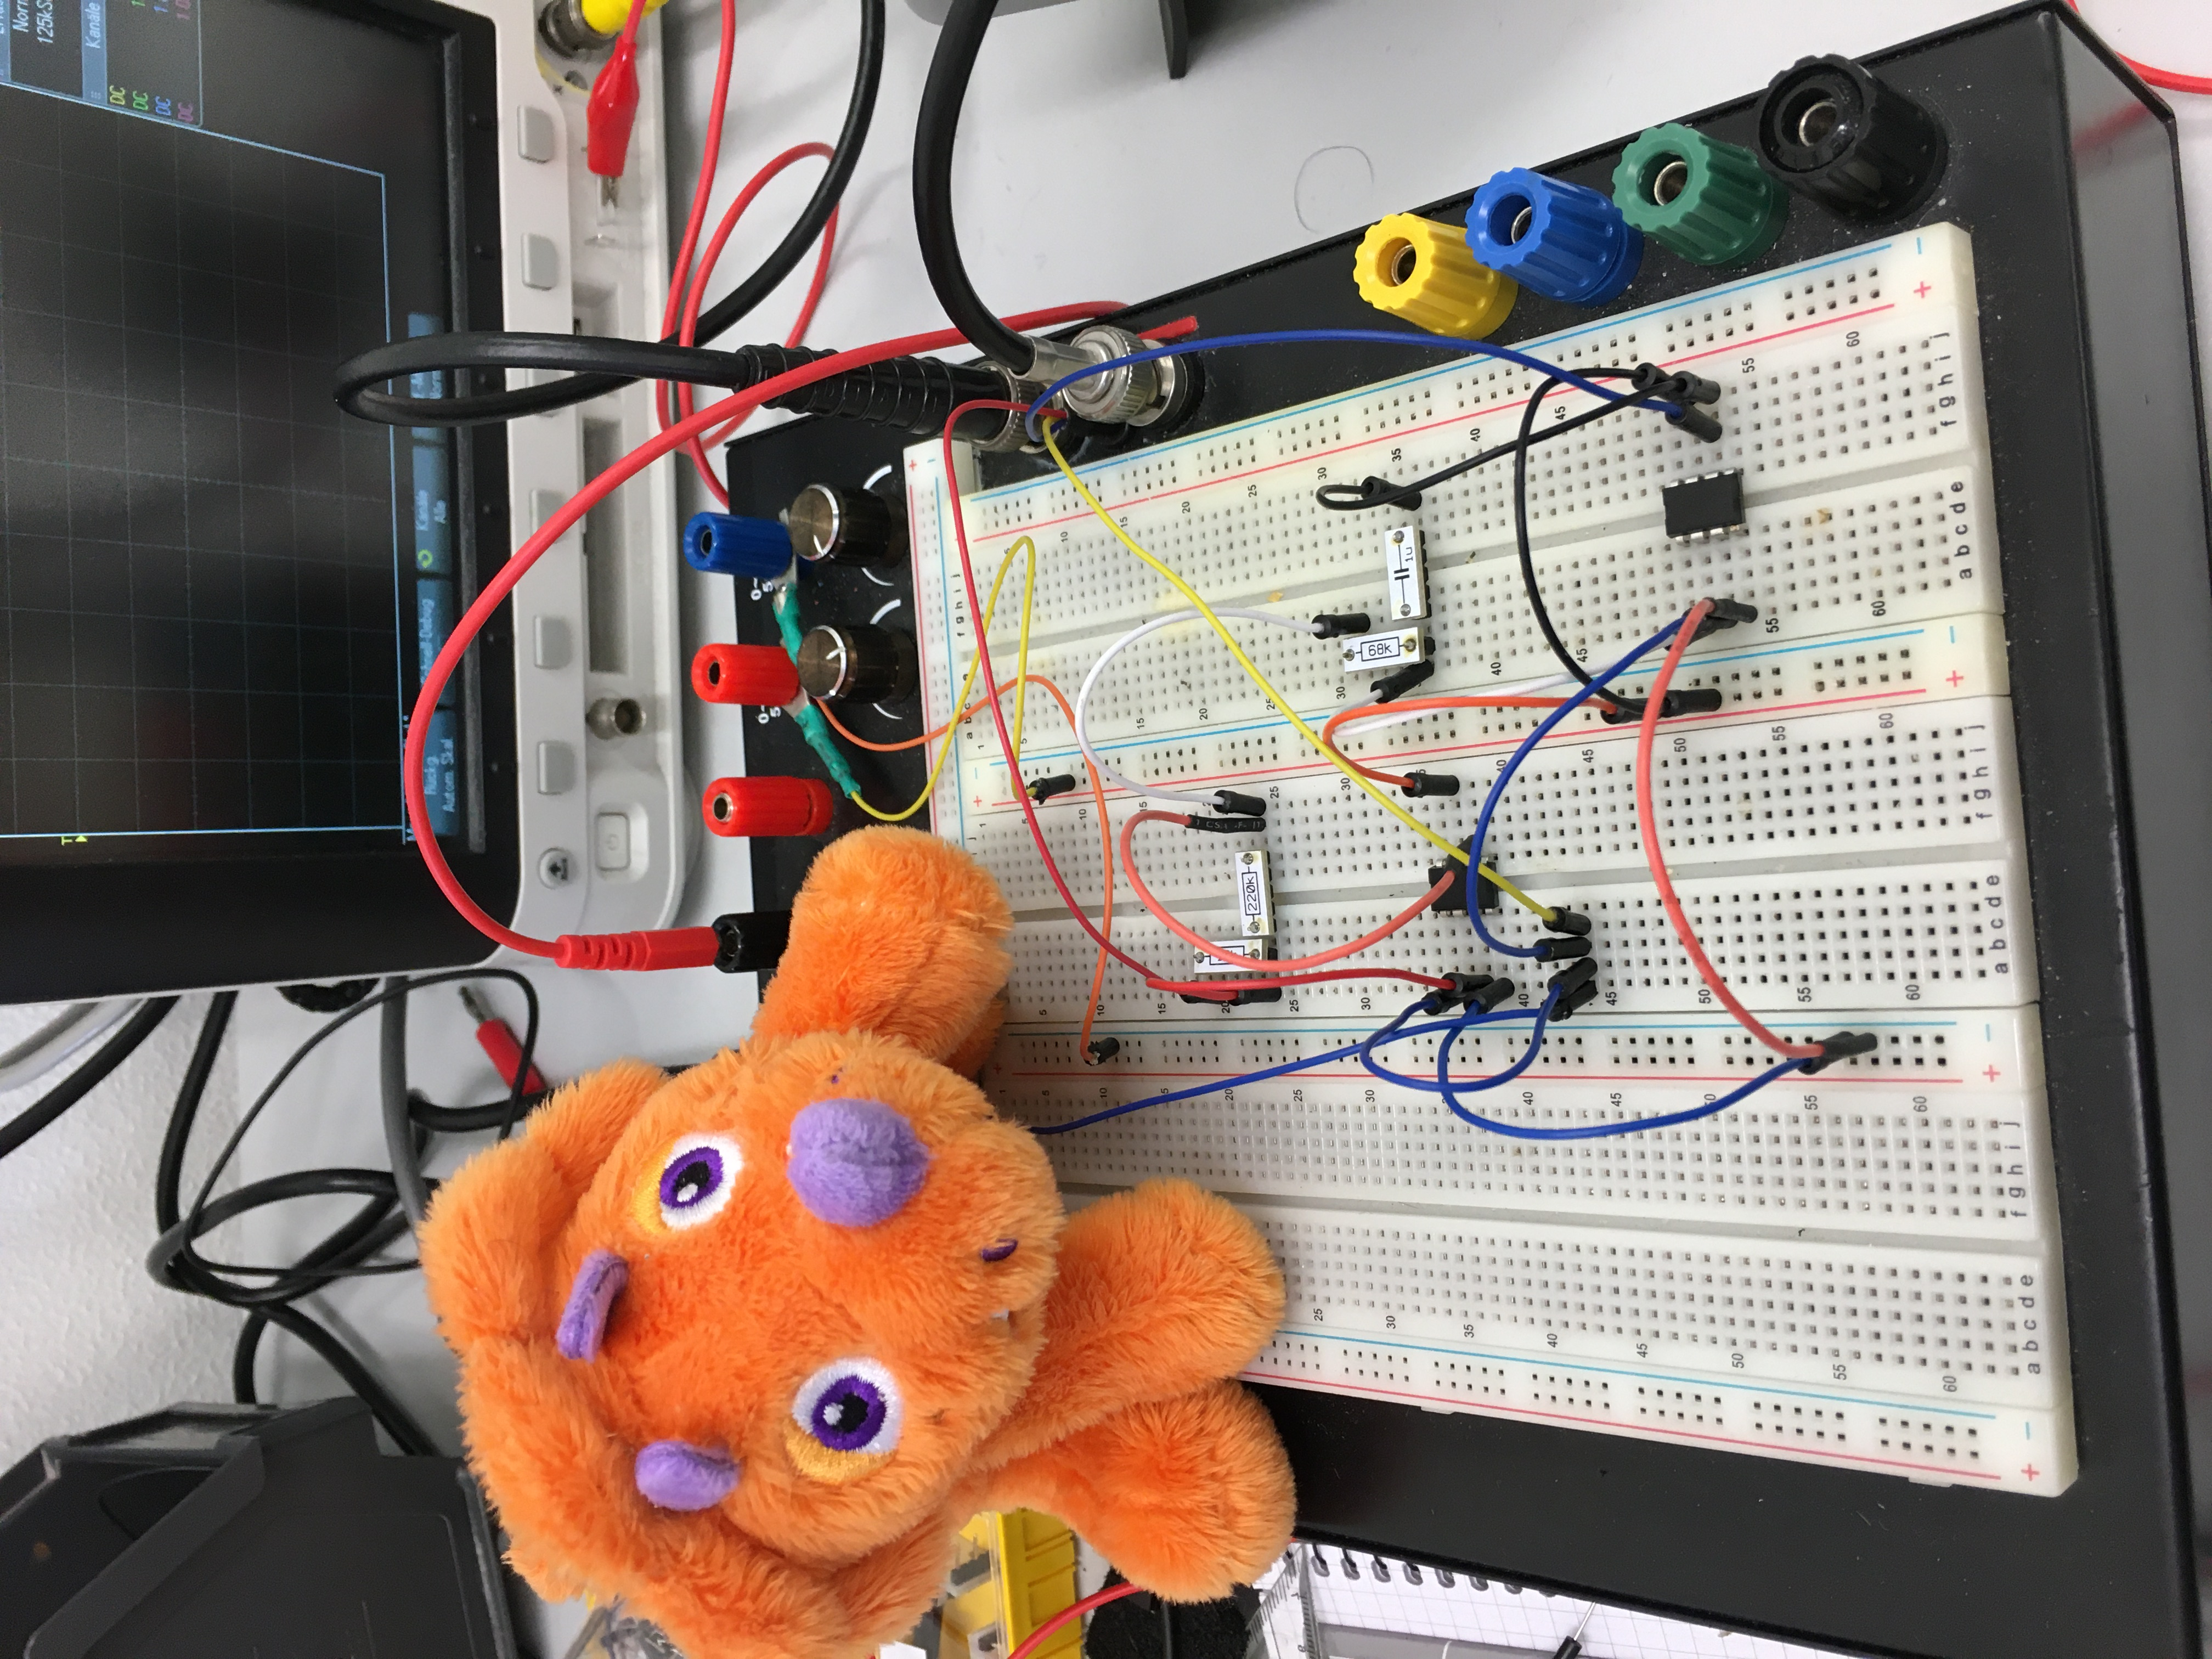
\includegraphics[scale=0.03]{ressources/aufbau.JPG}
  \caption{Versuchsaufbau zur Signalgeneratorschaltung.}
  \label{aufbau}
\end{figure}
\noindent Für die Schaltung zum invertierenden Linearverstärker werden die
Widerstände $R_1 = \SI{1}{\kilo\ohm}$ und $R_2 = \SI{100}{\kilo\ohm}$
verwendet. Die Betriebsspannung des Operationsverstärkers vom Typ LM741
liegt im Spannungsbereich von $U_1 = -\SI{15}{\volt}$ bis $U_2 = \SI{15}{\volt}$
\cite{datenblatt}. Für die Messungen wird eine Eingangsspannung
$U_e = -\SI{50}{\milli\volt}$ angelegt. Die Frequenz wird über mehrere Dekaden
variiert, das Eingangssignal ist dabei sinusförmig. Neben der Ausgangsspannung
wird die Phasenverschiebung zwischen Eingangs- und Ausgangssignal mit dem
Oszilloskop gemessen. Zu beachten ist, dass das Verstärkungssignal während der
Durchführung unverzerrt ist. Die Messung wird für verschiedene Widerstände
zweimal wiederholt. \\
\noindent Der Umkehr-Integrator wird mit dem Widerstand $R = \SI{10}{\kilo\ohm}$
und einem Kondensator der Kapazität $C = \SI{100}{\nano\farad}$ realisiert.
Die gewählte Zeitkonstante ist dabei durch Untersuchung der Proportionalität
zwischen Ausgangsspannung und dem Kehrwert der Frequenz (sinusförmiges
Eingangssignal) zu prüfen. Gemessen werden bei dieser Schaltung die Eingangs-
und Ausgangsspannungen in Abhängigkeit von der Frequenz. \\
\noindent Analog zum Umkehr-Integrator wird die Messung des invertierenden
Differenzierers durchgeführt. Dazu wird der Widerstand durch einen Kondensator
der Kapazität $C = \SI{20}{\nano\farad}$ und der Kondensator der vorherigen
Schaltung durch einen Widerstand $R = \SI{100}{\kilo\ohm}$ ersetzt. \\
\noindent Im Anschluss daran wird eine nicht-invertierende
Schmitt-Trigger-Schaltung gemäß \autoref{fig:07} aufgebaut. Für die
Widerstände gilt $R_1 = \SI{10}{\kilo\ohm}$ und $R = \SI{100}{\kilo\ohm}$.
Zu beachten ist hierbei die Vertauschung des nicht-invertierenden Signaleingangs
mit dem invertierenden Signaleingang. In Millivolt-Schritten wird ausgehend vom
Startwert $U = \SI{0}{\volt}$ die Amplitude des sinusförmigen Eingangssignals
erhöht und mithilfe des Oszilloskops die Amplitude ermittelt, bei welcher
die Schaltung zu kippen beginnt. \\
\noindent Nachdem die Kippspannung ermittelt wurde, wird hinter dem
Schmitt-Trigger ein Umkehr-Integrator auf das Steckbrett aufgesteckt. Die
Frequenz und Amplitude der erzeugten Schwingung werden mit dem Oszilloskop
untersucht.
